\chapter{Background}\label{chap:background}
This chapter briefly introduces the theoretical and practical components
involved in design and implementation of the Dual programming language and its
environment. 

\section{Web technologies}
As stated in the introduction, one of the main design goals of the system is usability.
%\js{Może rozwinąć myśl?  Chodzi o dostępność dla osób które nie znają się w ogóle na programowaniu? O dostepność dla osób które znają już JavaScript?}
This is accomplished in practice by building it on top of the most accessible and ubiquitous platform -- the web platform\cite{web_platform}\footnote{Also referred to as the \textit{open} web platform\cite{open_web_platform}}.

The language's interpreter and development environment are intended to work with
and are built on web technologies: JavaScript, HTML5 and CSS. The prototype
implementation makes use of Node.js, a server-side JavaScript runtime\cite{nodejs_site} and
CodeMirror, a JavaScript library which provides basic facilities for the text-based code editor part of the system\cite{codemirror_site}. This part is modeled after modern web-oriented code editors with similar design philosophy\cite{js_text_editors_wikipedia}, such as Visual Studio Code\cite{vscode_site}, Brackets\cite{brackets_site}, Atom\cite{atom_site} and many others.

\subsection{JavaScript}
The JavaScript programming language was created by Brendan Eich for Netscape\cite[Introduction]{ecmascript}, the company which created the Netscape Navigator web browser. There is a line of evolution that leads from Netscape and its browser to Mozilla and Firefox\cite{netscape_mozilla, mozilla_story}. The language was developed in 10 days in April 1995\cite{js_ten_days}.

Despite significant design flaws, JavaScript has became \textit{one of} the most\cite{tiobe. pypl}, if not \textit{the most}\cite[Section~Most Popular Technologies per Dev Type]{so_developer_survey_2016}\cite{redmonk} popular programming languages in the world. In this section I will briefly look at some of the probable reasons for that from a programming language design perspective.

On the surface, JavaScript has a familiar curly-brace syntax known from C or Java.

From a programming language design perspective, JavaScript has many great
features, borrowed from other excellent languages\cite[Section~4~Overview]{ecmascript}, most notably:
\begin{itemize}
   \item Scheme, one of two main dialects of Lisp\cite{r7rs}. It is a minimalist, but very extensible functional programming language. The features drawn from this language include first-class functions (treating functions as values), anonymous functions (also known as lambdas or function literals) and lexical closures.
   \item Self, a pioneering prototype-based \acrlong{oop} language\cite{self_handbook}, which evolved from Smalltalk-80\cite{smalltalk_history}. It introduced the concept of prototypes, which is an approach to \acrshort{oop}, where inheritance is implemented by reusing existing objects instead of defining classes. Prototype-based programming is the feature that JavaScript adopted from this language.
\end{itemize}
The two above languages are characterized by a very minimalist nature

The final advantage of JavaScript is the fact that it is distributed with a ubiquitous environment of the web browser. This makes the language straightforward for developers to use.
Easy to get started -- attract novice developers
Reach billions of users\cite{internet_stats}

The above mixture turns out to create a very powerful and usable language.

\subsubsection{Concurrency model}
In the context of the concurrency model, the JavaScript runtime conceptually
consists of three parts: the call stack, the heap and the message queue. All
these are bound together by the event loop\cite{mdn_concurrency}, which is the crucial part of this model.  An iteration of this loop involves the following steps:
\begin{enumerate}
	\item Take the next message from the queue or wait for one to arrive. At
          this point the call stack is empty.
	\item Start processing the message by calling a function associated with
          it. Every message has an associated function. This initializes the
          call stack.
	\item Processing stops when the stack becomes empty again, thus
          completing the iteration.
\end{enumerate}

This means, at least conceptually, that messages are processed one by one, in a single thread and an executing function cannot be preempted by any other function before it completes. In practice this is more complicated and there are exceptions to these rules. But this explanation is sufficient for further discussion.

This model makes reasoning about the program execution very straightforward, but
is problematic when a single message takes long to execute. This problem is
observed e.g. when web applications cause browsers to hang or display a
dialog asking the user if he wishes to terminate an unresponsive script.

For this reason it is best to write programs in JavaScript that block the event
loop for as short as possible and divide the processing into multiple messages.

This concurrency model is called the \textit{event} loop, because the messages are added to the queue any time an event occurs (an has an associated handler), such as a click or a scroll. In general input and output in JavaScript is performed asynchronously, through events, so it does not block program execution.

\section{Programming language design and implementation}
A very important family of programming languages and one which had the most
influence on the design of Dual is the Lisp family. In this thesis I use the
singular form ``Lisp'' to refer to the whole family rather that a concrete
dialect or implementation, such as Common Lisp or Scheme.

Lisp is characterized by a very minimal syntax, which relies on Polish (prefix)
notation for expressions and parentheses to indicate nesting. There are only
expressions and no statements in the language. This means that every language
construct represents a value. There's also no notion of operator precedence.

The two core components of a Lisp interpreter are the \texttt{apply} and
\texttt{eval}
functions\cite{sicp_meta}\footnote{\url{http://c2.com/cgi/wiki?EvalApply}}. The
former takes as arguments another function and a list of arguments and applies
this function to these arguments. The latter takes as arguments an
\texttt{expression} and an \texttt{environment} and evaluates this expression in
this environment. The typical implementation of \texttt{eval} distinguishes
between a few types of expressions. The essential are:
\begin{itemize}
	\item Symbols (also known as identifiers or names) --
          e.g. \texttt{velocity} -- these are evaluated by looking up the value
          corresponding to the symbol in the environment, so \texttt{velocity}
          might evaluate to \texttt{10} if it is defined as such in the
          \texttt{environment}
	\item Numbers (or number literals) -- e.g. \texttt{3.2} -- these
          evaluate to a corresponding numerical value
	\item Booleans (boolean literals) -- \texttt{true} or \texttt{false} --
          evaluate to a corresponding boolean value
	\item Strings (string literals) -- e.g. \texttt{"Hello, world!"} --
          evaluate to a corresponding string value
	\item Quoted expressions -- e.g. \texttt{'(+ 2 2)} -- a quoted
          expression evaluates to itself; in other words a quote prevents an
          expression from being evaluated
	\item \textit{Special forms} or \textit{primitives}, which are
          expressions that have some special meaning in the language. These are
          the basic building blocks of programs. For example:
	\begin{itemize}
		\item \texttt{if}, the basic conditional expression and other
                  flow control expressions; the special meaning of these is that
                  they evaluate their arguments depending on some condition
		\item \textit{lambda} expressions -- essentially function
                  literals, which consist of argument names and a body
		\item \textit{definition} and \textit{assignment} expressions;
                  these modify the environment; usually they treat their first
                  argument as a name of the symbol in the environment, so it is
                  not evaluated; the second argument is evaluated and its value
                  is associated with the symbol
	\end{itemize}
\end{itemize}

\js{Brakuje mi tu gdzieś jasnego powiedzenia, że listy którymi manipuluje lisp
  mogą być zarówno przetwarzane jako dane, jak i wykonywane jako kod.  Chyba że
  nie jest to szczególnie istotna własność z punktu widzenia Dual -- wtedy można
  to pominąć.}

For detailed explanation please refer to \cite{sicp_meta}.

\subsection{Syntax}
The term ``\acrlong{ast}'' refers to a tree data structure that is often \js{skreśliłbym often} built
by parsers of programming languages to represent syntactic structure of source
code in an abstract and easily traversable and manipulable way. In the simplest
form, in expression-only languages such as Lisp each node of such tree
represents a single expression. The tree is abstract in the sense that it does
not necessarily contain all the syntax constructs that occur in the source code
or encodes them in some ``abstract'' way. In case of Lisp, there's no need to
store or represent bracketing characters \texttt{()} in the AST, as nesting is
inherent in the structure itself.

In theory, a programming language does not require a text representation and
could be defined only in terms of a data structure such as a syntax
tree. Practically, for a language to be useful, it needs to come with an
editable representation that provides a convenient way for a programmer to
construct programs. Currently the most successful representation for that is the
human-readable text-based representation, which evolved from more primitive and
less convenient representations, such as punched cards.

Constructing programs with this \js{this -> text} representation can be done with any text editor.

This means that the representation is largely independent of a tool, which is an
advantage. Any application capable of editing text can theoretically be used to
edit any source code (ignoring details such as encoding, etc.). Such
applications are universally available, so source code stored in text files can
be edited freely on any platform with any tool.

But for complex programs a simple text editor quickly becomes inconvenient and a
more specialized one is preferable. Such code editors introduce various features
that greatly improve the convenience of working with a text-based representation
of a programming language. For example:
\begin{itemize}
	\item Automatic structuring of the text to emphasize blocks of code
          (autoindentation)
	\item Highlighting different syntactic constructs with different colors
	\item Context-based autocompletion
	\item Autoclosing of bracketing characters
	\item Automatic correction of errors
	\item The ability to fold distinct blocks of code
	\item Advanced navigation through the code: jumping to declarations,
          definitions, other modules or files
	\item Etc.
\end{itemize}
Most of these features require that the editor makes use of a parser to
recognize the syntactic structure of a program.

Other advantages of a text representation, that stem from the multitude of ways
that raw text can be manipulated and processed:
\begin{itemize}
	\item Find and replace with regular expressions
	\item Selecting/processing many lines or even blocks of text
	\item Editors often treat the source as a 2D grid of characters; each
          row and column of such grid can be numbered
	\item Debuggers, compilers and other elements of a programming language
          system can use row and column numbers in error messages
	\item Version control systems can easily diff and keep track of changes
          in text files
\end{itemize}


\subsection{Visual programming languages}
An alternative representation is the one employed by visual programming
languages. Such languages are usually tied to a particular editor, which allows
the programmer to edit the source code with a mouse rather than the
keyboard. That is instead of typing in streams of characters to be parsed and
assembled into a structural form, he inserts, arranges and connects together
distinct visual elements to produce such a structure. Thus I contend that visual
programming can be defined at the lowest level as manipulating a visual form of
a language's syntax tree.

The design of the visual representation for my language involved a rough survey
of visual programming languages. In this section I will briefly describe the
results obtained from this survey\footnote{A formal study of visual programming
  languages, proper classification in terms of statistics and methodical
  examination are not the focus of this thesis. \js{No ja bym jednak tego nie pisał i zamiast tego zrobił solidny przegląd literatury.}}.

I classified each of nearly 160 languages listed in \cite{snapshots}, according
to type of their visual representation, to one of three categories:
\js{Może Pan wyjaśnić czym się różni 1 od 2?  Mam poczucie, że wrzucenie obrazków pokazujących jedno i drugie mogło by pomóc.}
\begin{enumerate}
    \item Line-connected block-based, exemplified by Blueprints Visual
    Scripting system of Unreal Engine 4\cite{blueprint}: about 66\%
    \item Snap-together block-based, exemplified by MIT Scratch\cite{scratch, scratch_wikipedia}
    \item Other
\end{enumerate}


\begin{figure}[h!]
\centering 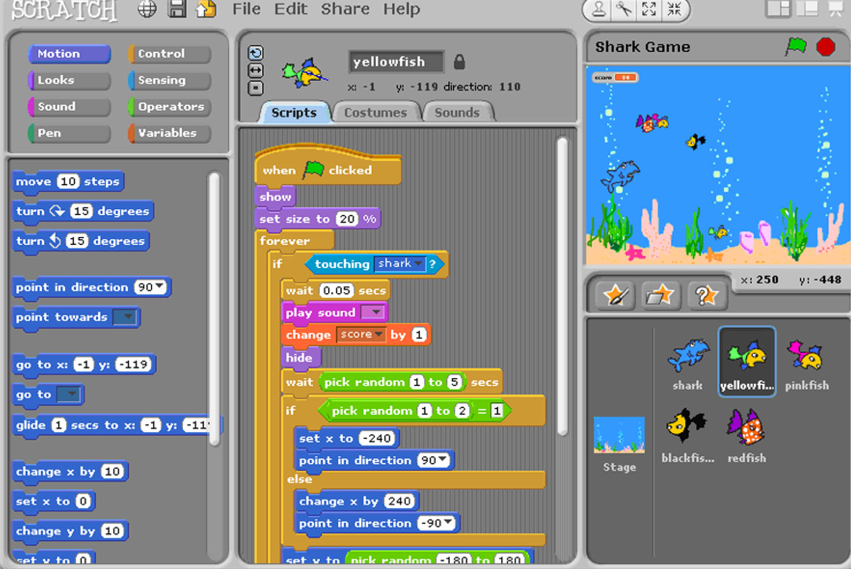
\includegraphics[width=0.9\textwidth]{scratch}
\caption{ MIT Scratch programming language editor\protect\footnote{ Screenshot
        from \url{
            http://mypad.northampton.ac.uk/12406702/files/2013/05/Screen-Shot-2013-05-02-at-23.19.19-1s0qp26.png
        } } }
\label{fig:scratch}
\end{figure}

\begin{figure}[h!]
\centering 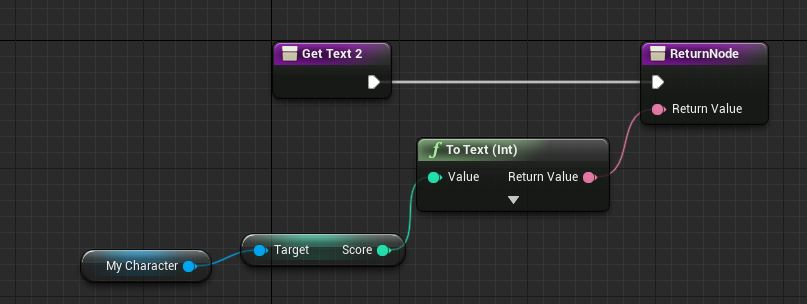
\includegraphics[width=0.9\textwidth]{blueprint}
\caption{Blueprints Visual Scripting\protect\footnote{Screenshot from
        \url{https://docs.unrealengine.com/latest/images/Engine/Blueprints/HowTo/BPHT_6/GetScore.jpg}}}
\label{fig:blueprint}
\end{figure}


Additionally, I associated each language with a number $s \in [0, 3]$, which
descirbes its ``structure factor''. This tries to quantify my subjective
assessment of the readability of the representation compared to familiar text
representation ($s = 3$)\footnote{This is based solely on the screen shots from
  the editors. For example, if it appears that the representation consists of
  scattered blocks, connected by lines and the layout seems to be arranged by
  the user, with no automatic structuring by the editor, $s$ will be low.}.
\js{Może po prostu napisać że im więcej tym lepiej?}

Below I present the results of this classification. The elements are structured
as follows: name of category -- percentage of languages that fall into the
category -- the average ``structure factor'' $s$ for the category This yielded
the following results:
\begin{enumerate}
    \item Arrow/line connected blocks -- 66\% -- 0.61
    \item Snap-together blocks -- 11\% -- 2.4
    \item Other representations -- 23\% -- 1.39, notably:
    \begin{enumerate}
        \item Lists -- 2.5\% -- 2
        \item GUI -- 2.5\% -- 1
        \item Nested -- 2.5\% -- 2
        \item Enhanced text -- 2.5\% -- 2.75
        \item Timeline -- 2\% -- 1.17
        \item \textit{The remaining 11\% are various other representations:
          in-game \acrshort{vpl}s, hybrid, specialized, esoteric, etc.}
    \end{enumerate}
\end{enumerate}
\js{No ja mam poczucie, że powyższe jednak wymagają bliższego wyjaśnienia.}

Taking into account the above and looking at the most popular visual programming
languages\footnote{I was not able to find and am not aware of any official or
  even unofficial ranking of popularity of visual programming languages, but
  analyzing the top hits when google searching the phrase ``visual programming
  language'' in combination with
  \url{https://en.wikipedia.org/wiki/Visual_programming_language} and my
  personal experience suggest that we can find these among the most popular: MIT
  Scratch Unreal Engine 4's Blueprints}
\js{Urwane zdanie?}

\js{Coś jest nie tak z początkiem tego zdania}
From this and a I drew the conclusion that there are basically two main
representations. A flowchart-like representation, exemplified by the Blueprints,
with blocks connected by lines or arrows, which usually leaves the layout of the
program source completely to the user, providing no automatic
structuring. Another representation is exemplified by MIT Scratch. There, the
code is represented and manipulated in terms of snap-together blocks, similarly
to a jigsaw-puzzle. This representation is self-structuring and is designed to
resemble a faimiliar text-based, indent-structured representations.

The advantages of the first representation is that it clearly separates
\js{Znowu coś nie tak ze zdaniem}

The lack of support for automatic structuring, which is an essential feature of
modern text-based code editors is obviously a regression.
\js{To zdanie wydaje mi się całkowicie wyrwane z kontektsu.}

To design a visual representation that can be an improvement over the text-based
representation all the advantages of the latter need to be kept.

\js{Jakiś chaos się tutaj wkradł. Może czytam pracę trochę za szybko, ale nie przypominam sobie jakie były te zalety tekstowej reprezentacj. Pamiętam że były cechy, ale bez podziału na zalety i wady.}

\section{Programming discipline}
\js{mam poczucie, że ten podrozdział jest nie na miejscu. Lepiej napisać to gdzieś przy opisie implementacji}
The prototype was implemented largely in the spirit of exploratory programming:
``the kind where you decide what to write by writing
it.''\footnote{\url{http://arclanguage.org/}}.

This approach in combination with a dynamic and flexible language like
JavaScript enables one to quickly transform ideas to working prototypes and
shape them as one goes along. But the usefulness of this method is limited, as
it may quickly produce fairly low-quality code, as it is not focused on future
maintainability.
